\chapter{The LHC and ALICE}\label{ch:alice}

\section{Overview of The LHC}\label{sec:LHC}
The Large Hadron Collider (LHC)\cite{doi:10.1142/S0217751X13300354} is a circular particle accelerator located on the Franco-Swiss border near the city of Geneva.  It is operated by the European Organization for Nuclear Research (CERN) and has carried out proton-proton (pp), lead-proton (pPb), and lead-lead (PbPb) collisions at center of mass energies of  0.9-14 TeV, 5.0 TeV, and 2.76-5.5 TeV, respectively.  The LHC is approximately 17 miles in circumference and is located 200 meters underground, inside the old accelerator tunnel used by the Large Electron-Positron\cite{Taylor:2017edx} collider of the 1980's.  There are over 8000 physicists and engineers making up the four main experiments at the LHC: ATLAS\cite{Aad:2008zzm}, CMS\cite{Chatrchyan:2008aa}, LHCb\cite{Alves:2008zz}, and ALICE\cite{Aamodt:2008zz}.   Numerous physics results have been published, with the most famous being the discovery of the Higgs boson in 2012\cite{Chatrchyan:2012xdj}\cite{Aad:2012tfa}.

\begin{figure}[h]
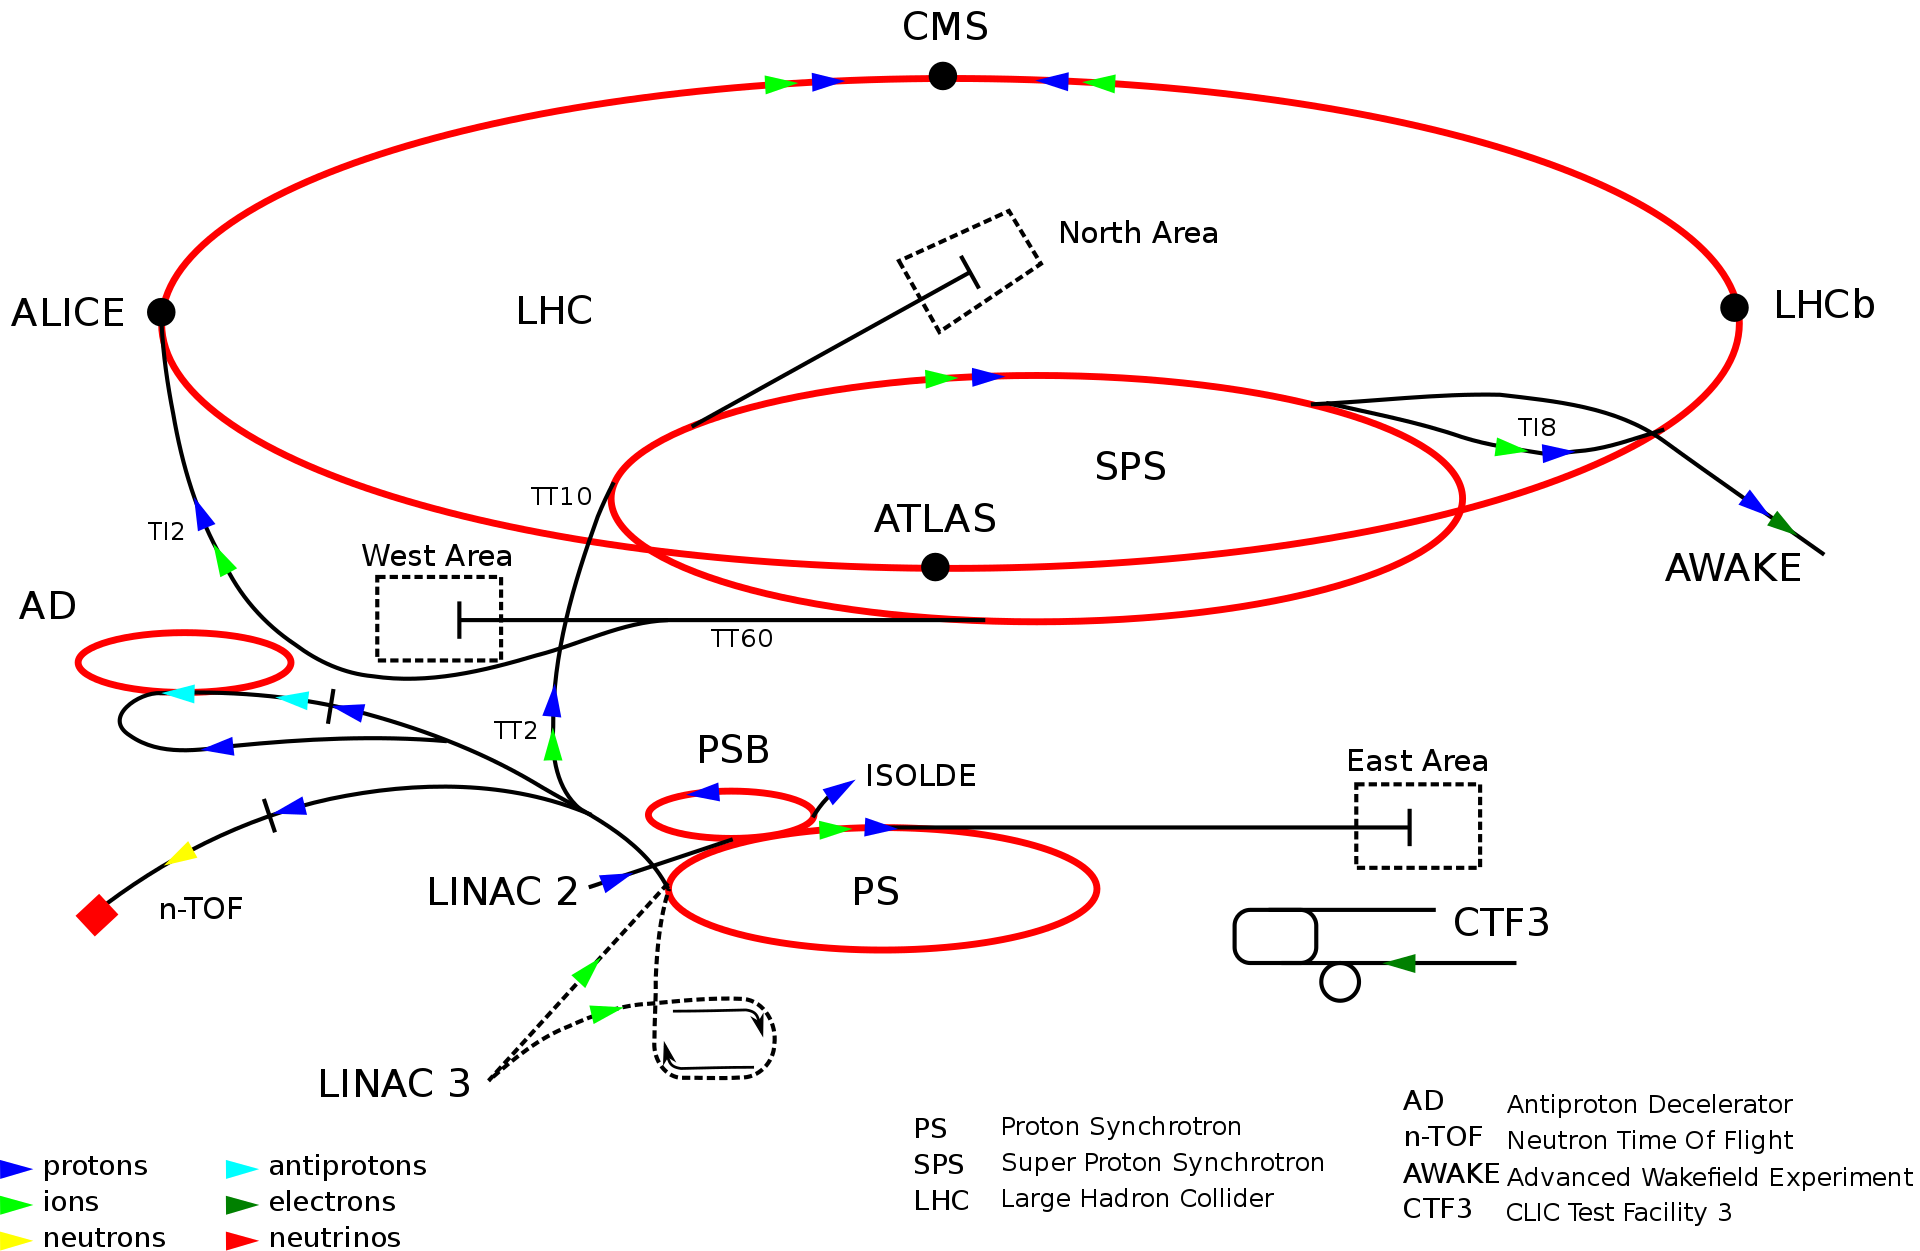
\includegraphics[width=15.0cm]{1920px-Cern-accelerator-complex}
\centering
\caption{LHC accelerator complex.  The four main experiments are shown in their relative locations\cite{Mobs:2197559}.}
\label{fig:AccComp}
\end{figure}

Figure \ref{fig:AccComp} shows a schematic of the LHC along with the pre-accelerators that help to accelerate protons and ions to their final energies before a collision at one of the four experimental interaction points (IP).  Protons are injected into the LHC in groups called `bunches'.  Every bunch is comprised of about 120 billion protons with about 50 nanoseconds between the arrival of the next bunch.  The bunch scheme during the heavy-ion run is reduced to 200 nanoseconds due to the high multiplicity of the events and additional computational resources needed. 

\subsubsection{LHC Operations}
The LHC first attempted particle collisions in September of 2008.  The initial ramping up of the super conducting magnets led to mechanical failure of the helium pipes inside of the LHC beam line.  This fault caused the LHC to remain shut down for over a year while the accelerator was repaired and new safety procedures were implemented. The first successful collisions occurred in 2009 with proton collisions at a reduced energy of 0.9 TeV.  2010 marked the beginning of a new era in the high energy frontier with proton collisions at a record setting 7 TeV.  The only other major fault that has occurred was in the summer of 2016. A stone marten chewed through a high voltage line in a power transformer on a ground level building at the LHC.  The LHC went offline for about a week while repairs occurred and quickly resumed the physics program.  Unfortunately, the marten did not survive.

The typical operating year at the LHC allows for any repairs or upgrades on the experiments to be performed during the offline period for the first few months.  After the offline period, the proton physics program begins and lasts until approximately mid-November.  The heavy-ion program begins after the proton physics run and lasts until the first week of December, after which the LHC shuts down for the remainder of the year.  

From 2014 until early 2015 the LHC was shutdown for major renovations and upgrades to the accelerator and a number of sub-detectors on each experiment. This was known as long shutdown 1 (LS1).  Since the end of 2018, the LHC has been in another long shutdown (LS2), which aims at upgrading the accelerator to a high luminosity, Hi-Lumi.  This will be discussed in detail along with the upgrades to ALICE in Chapter \ref{ch:tpcu}.

\subsubsection{LHC Accelerator Complex}\label{sec:LHCop}
The LHC accelerator complex is a succession of particle accelerators that increase the energy of particles before they are injected into the next accelerator.  Hydrogen atoms are first passed through a high voltage environment that strips any electrons from around the proton.  Once the protons are stripped of their electrons, they are injected into the linear accelerator (LINAC).  The LINAC uses radio frequency cavities to accelerate particles to 50 MeV before they enter the first circular accelerator the Proton Synchrotron (PS).  The PS begins to focus the protons into bunches and further accelerates them to 1.4 GeV before the the beam enters the Super Proton Synchrotron (SPS).  The SPS accelerates the particles to 450 GeV.  The beam is then injected into the LHC and accelerated to the final collision energy.  Afterwards the beam gets `squeezed', or tightly focused, with a series of quadrupole magnets.  The final step is to `adjust'  the beam to overlap with the counter-rotating beam at the four interaction point (IP) were the main LHC experiments are located.  Once the adjust phase is completed, collisions will occur at each experiment and data  collection begins.  This entire process from stripping the electrons to collisions in each IP takes 20 minutes.

In order for the beam parameters to be maintained in the LHC, numerous dipole and quadrupole magnets are used to accelerate, focus, and bend the particle beams.  The magnets use a superconducting niobium-titanium alloy that is maintained at an operating temperature of 1.9 K using helium-4.  Upgrading these magnets is one of the major goals during LS2 as part of the Hi-Lumi upgrade of the LHC\cite{Fabjan:2011jb}.


\section{The ALICE Experiment}
A Large Ion Collider Experiment (ALICE) is a general purpose detector that covers a solid angle of 4$ \pi$ around the IP.  It is 26 m long, 16 m high, 16 m wide, and weighs approximately 10,000 tons\cite{Fabjan:2011jb}.  Like many other large scale detectors, ALICE is made up of 18 sub-detectors that perform tracking, particle identification (PID), timing, vertex reconstruction, and calorimetry.  


Figure \ref{fig:alice} shows the ALICE detector with human figures to set the scale.  Figure \ref{fig:ITS} shows the area closest to the interaction point with the TZERO, VZERO, Inner Tracking System and Forward Multiplicity Detector.  These detectors give basic information on the collision such as vertex location, centrality, and timing.   Further out from the central region are a number of tracking detectors, like the Time Projection Chamber and Time-of-Flight detectors, which focus on  measuring charged particle momentum and PID.  Next are the calorimeters that measure particle and jet energies, such as the Electromagnetic Calorimeter, Photon Spectrometer, and  Dijet Calorimeter.  All of these sub-detectors are housed in the L3 magnet, seen as the red octagon in Figure \ref{fig:alice}.   The L3 magnet provides an approximately uniform magnetic field of 0.5 T over the central area of ALICE and helps ensure the high PID performance ALICE has over a wide kinematic region\cite{Gligorov:2018vkc}.  At high rapidity, there is a muon tracker and trigger for muon identification.  The following sections give a more detailed discussion of the sub-detectors used for this analysis

\afterpage{%
\begin{figure}[h!]
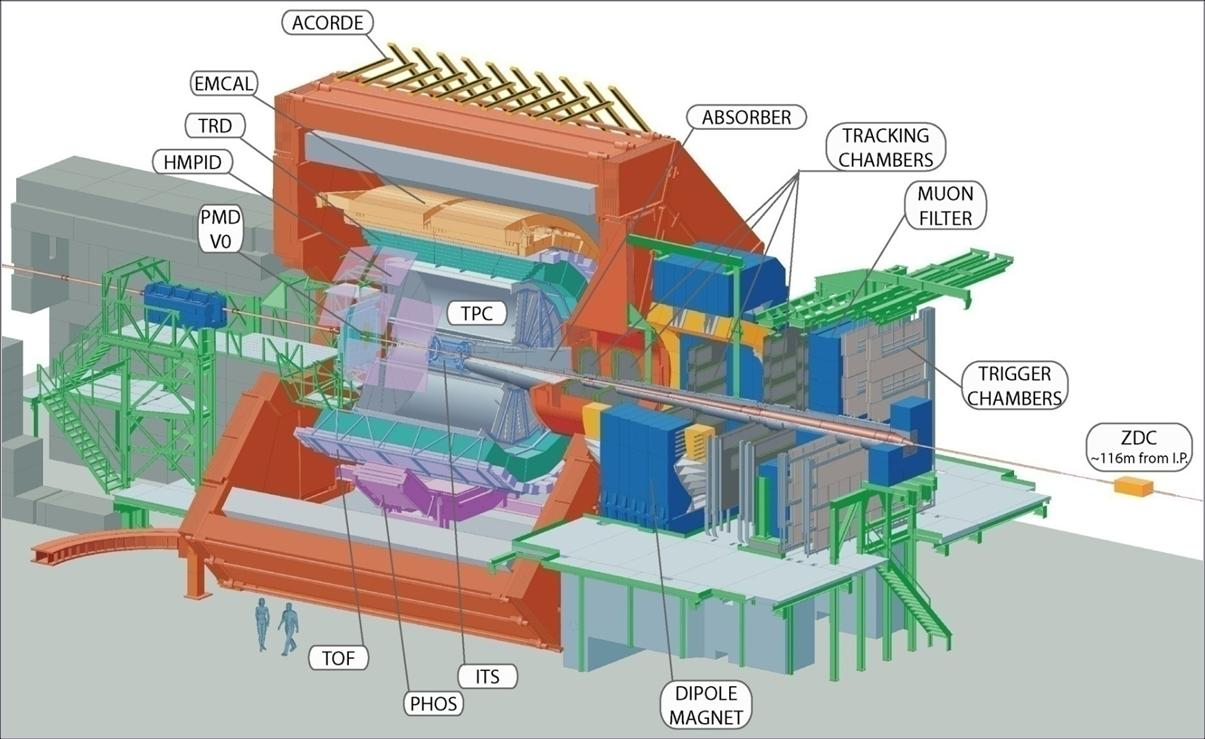
\includegraphics[width=\linewidth]{ALICE-event-b}
\centering
\caption{The ALICE Detector at CERN\cite{Alberico:2011zy}.}
 \label{fig:alice}
\end{figure}

\begin{figure}[h!]
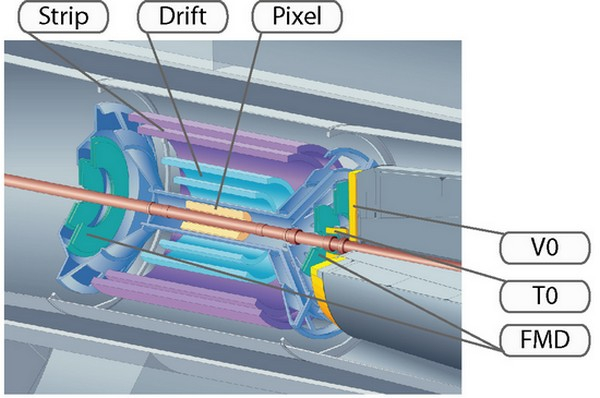
\includegraphics[width=10cm]{ITS}
\centering
\caption{ALICE tracker, multiplicity, timing, and vertex detectors located near the interaction point\cite{Alberico:2011zy}.}
 \label{fig:ITS}
\end{figure}
\clearpage
}

\subsubsection{TZERO}
The TZERO (T0)\cite{Bondila:2005xy} detector is a double layer Cherenkov counter located at 70 cm (T0A) and 370 cm (T0B) from the IP.  The T0 functions as a trigger and timing detector that determines the precise moment in time at which an event `starts' in the ALICE detector.  The timing information from the T0 is fed to other sub-detectors, like the Time-of-Flight and Time Projection Chamber detector, which is used for track reconstruction. in the case of the Time Projection Chamber  The T0 also gives feedback on the target luminosity of the ALICE experiment to the LHC operations center.  

\subsubsection{VZERO}
The VZERO (V0)\cite{Abbas:2013taa} detector is a double layer scintillator array and similar to the T0 is asymmetrically placed at a distance of 86 cm (V0A) and 329 cm (V0C) away from the primary IP.  It provides the `minimum bias' (Min Bias)\footnote{A Min Bias event is unsurprisingly defined as an event with the least amount of bias possible.  Events recorded with a Min Bias trigger attempt to not artificially prefer either diffractive or non-diffractive processes over one another\cite{Field:2011iq}.} trigger information for events and centrality information during the heavy-ion run.   Centrality\footnote{Centrality (c) is an estimation of the impact parameter (b) between the two colliding nuclei.  It is proportional to the cross-section and is given as $c = \frac{1}{\sigma_{inel}} \int^{b}_{0} db \frac{d\sigma}{db}$} is determined by measuring the multiplicity amplitude from the V0 and fitting these results to a Glauber\footnote{The Glauber model treats the nucleons composing a nucleus as hard shells, more can be found here \cite{Loizides:2016djv}.} distribution.  The V0 is also capable of precision measurements of the target luminosity in the ALICE detector.


\subsubsection{Inner Tracking System}\label{sec:its}
The Inner Tracking System (ITS)\cite{BEOLE20121062} is six layers of solid state silicon detectors.  Closest to the beam line are two layers of Silicon Pixel Detectors.  The next two layers are Silicon Drift Detectors and furthest from the beam line are two layers of Silicon Strip Detectors.  The main purpose of the ITS is to perform momentum measurements, PID, and vertex reconstruction of charged tracks.  PID\footnote{See Appendix \ref{ref:pid}} is performed by measuring the ionization energy, $\frac{dE}{dx}$, of charged particles as they traverse the detector\cite{Adam:2016acv}.  The ITS has a spatial resolution of 100 $\mu m$.  This allows for measurements of short lived hadrons by reconstructing secondary vertices, which is useful in measuring hadrons containing heavy quarks, bottom and charm.


%TPC

\subsubsection{Time Projection Chamber}\label{sec:tpc}

\begin{figure}[h]
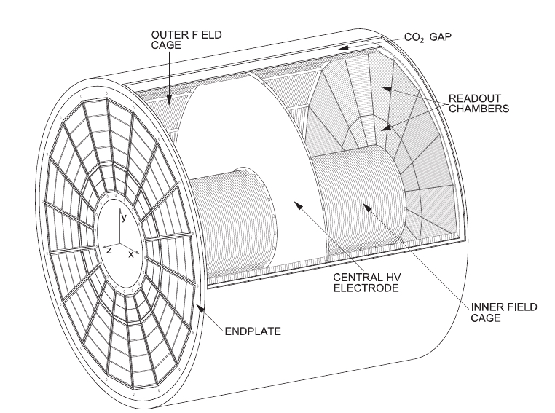
\includegraphics[width=12.0cm]{alice-tpc-schematic}
\centering
\caption{The ALICE Time Projection Chamber\cite{2010NIMPA.622..316A}.}
\label{fig:TPC}
\end{figure}

The Time Projection Chamber (TPC)\cite{2010NIMPA.622..316A} is a gaseous charged particle tracker and the largest of its kind in the world.  The TPC has full azimuthal coverage, a pseudorapidity acceptance of $ \left | \eta \right | \leq 0.7$, and a volume of 93 $m^{2}$.  Figure \ref{fig:TPC} shows a schematic of the TPC.  As charged particles traverse the drift volume of the TPC, they ionize the gas inside\footnote{The TPC has operated with $Ne-CO_{2}$ (90-10) and $Ar-CO_{2}$ (90-10) gas mixtures in the past}.  A central cathode in the TPC wth a voltage of 100 kV induces a uniform electric field of 400 V/m along the beam axis throughout the drift volume.  Ionized electrons will drift down to the cylindrical endcaps of the TPC where the read-out chambers (ROC) are located.  There are 18 ROCs on each side of the TPC which are further broken into an Inner Read Out Chamber (IROC) and an Outer Read Out Chamber (OROC).  

\subsubsection{The TPC Readout}\label{sec:tpcread}

\begin{figure}[h]
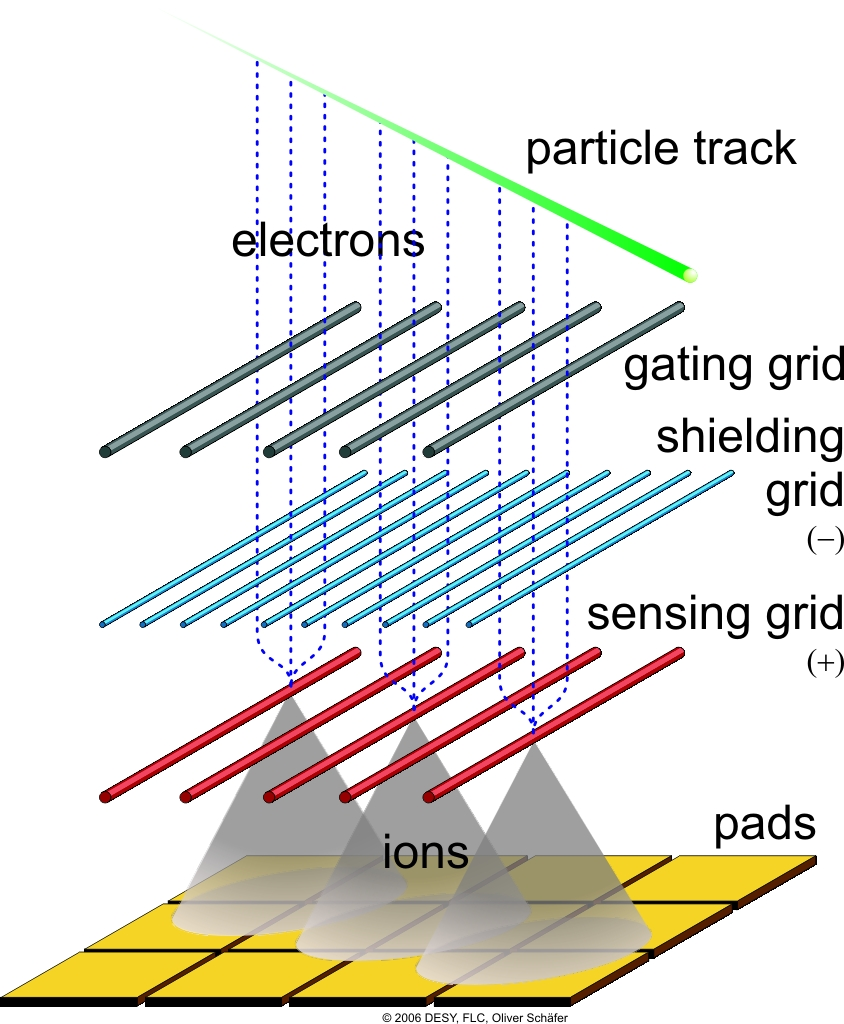
\includegraphics[width=9.0cm]{Wirereadout_eng}
\centering
\caption{The TPC readout region\cite{diener}.}
\label{fig:TPCreadout}
\end{figure}

The TPC incorporates a Multi-Wire Proportional Chamber (MWPC) design for amplification and copper pads for readout\footnote{There are 72 MWPCs and 500K copper pads in the ALICE TPC}. Ionized electrons created from charged particles take approximately 100 $\mu s$ to move from the drift volume to the readout region.  Once these electrons enter the readout region, they will undergo an amplification process with the MWPC, seen as the sensing grid wires in Figure \ref{fig:TPCreadout}.  This amplification process will turn the few dozen ionizated electrons generated from a charged particle into thousands of amplified electrons that are sensed by the cooper pads and read from the front-end electronics(FEE).  

Amplification using MWPCs has the disadvantage of creating thousands of ions known as `backflow ions' that can move back into the drift volume of the TPC.  The presence of backflow ions in the drift volume of the TPC will cause distortions in the uniform electric field of the TPC.  These distortions are known as `space-charge' distortions and will compromise the physics performance of the TPC.  In order to minimize the space-charge distortions, the TPC incorporates a gating grid\cite{Tangwancharoen:2016dqs}.  Once an event is detected in the readout electronics of the TPC, a high voltage is induced on the gating grid.  This will capture any backflow ions moving from the amplification region to the drift volume.  When engaged, the gating grid introduces a dead time as any ionization electrons from new events occurring in ALICE will also get captured.  The current configuration of the gating grid is designed to engage for 300 $\mu s$ after an event is first detected.  This has been shown to absorb approximately 99\% of the backflow ions created while preserving the TPC physics performance.  The dead time due to the gating grid along with the drift time for charged particles in the TPC limits the readout to 3.5 kHz.  Upgrading the triggered operation of the current TPC to a continuous readout for the Hi-Lumi upgrade of the LHC will be discussed in detail in Chapter \ref{ch:tpcu}.

\subsubsection{TPC Performance}\label{sec:tpcper}

In order to reconstruct the trajectory of a particle, an iterative process known as a Kalman filter approach is used.  The x, y coordinates, which are perpendicular to the beamline, are determined via the signal induced on the copper pads.  The z component, which is parallel to the beamline, is reconstructed using the timing information from the T0.  

\begin{figure}[h]
   \centering
      \subfloat[TPC momentum resolution]{\label{fig:figure-TPCb}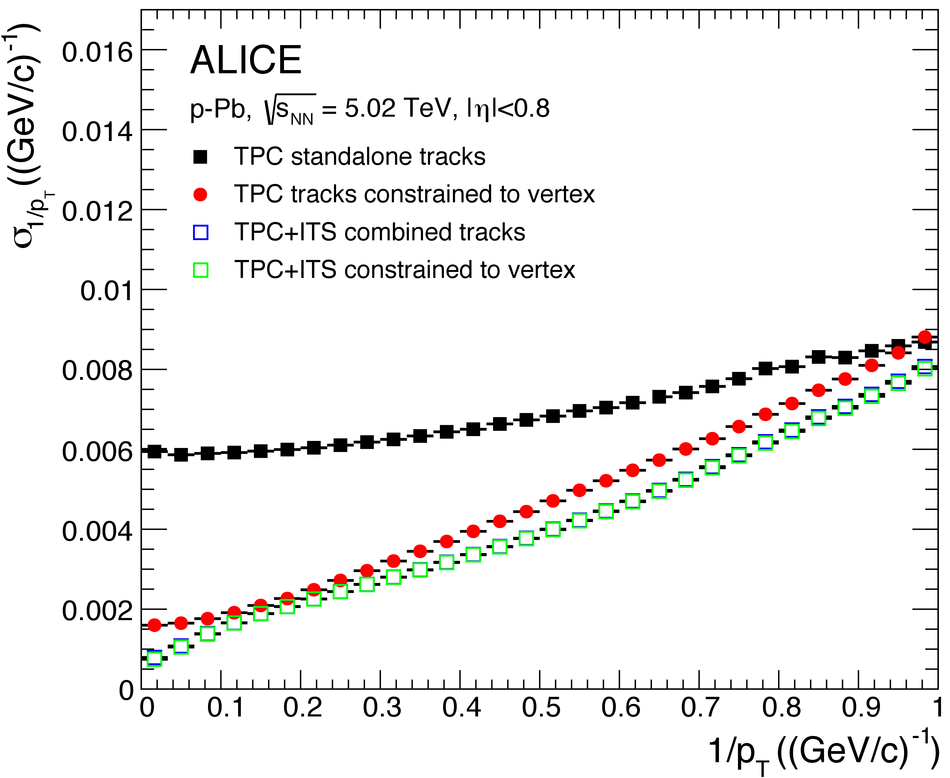
\includegraphics[width=3.0in]
     {PTresolution_vs_1Pt_pPb_2013_PerfPaper-8441}}
   \subfloat[ITS-TPC track matching efficiency]{\label{fig:trk-match}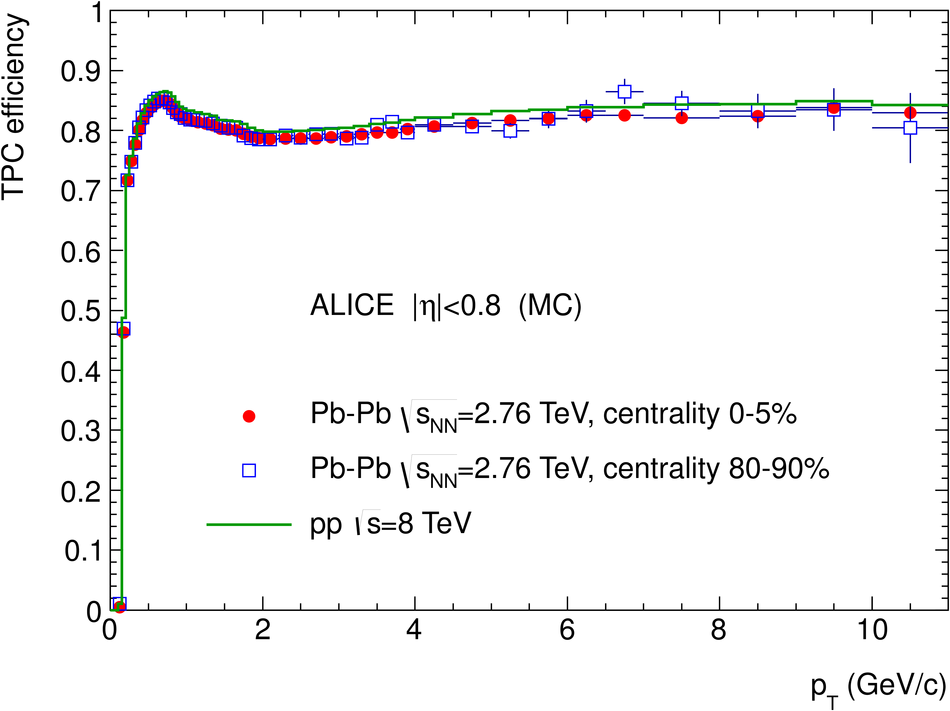
\includegraphics[width=3.0in]
     {tpc_abseff-8423}}
   \caption{TPC momentum and tracking resolution\cite{Abelev:2014ffa}.}
   \label{fig:multipart-TPC}
\end{figure}


The TPC has excellent momentum resolution between 150 MeV/\textit{c} to 100 GeV/\textit{c}\cite{LIPPMANN2012434}.  Figure \ref{fig:figure-TPCb} shows the inverse momentum resolution as being below 5\% in black.  The inverse momentum resolution was further improved to below 0.5\% over the full kinematic range by matching TPC tracks to ITS tracks and constraining those tracks to originating from the primary vertex region, red and green respectively.  The total efficiency between ITS tracks to TPC tracks is stable at about 80\%, as seen in Figure \ref{fig:trk-match}.



%EMCAL

\subsubsection{Electromagnetic Calorimeter}
The Electromagnetic Calorimeter (EMCal)\cite{1742-6596-293-1-012043} is a lead based sampling calorimeter located at a radius of 4.5 meters from the beam pipe.  It covers a pseudorapidity of $ \left | \eta \right | \leq 0.7$ and has azimuthal coverage of $ \Delta \phi = 107 \deg$.

\begin{figure}[h]
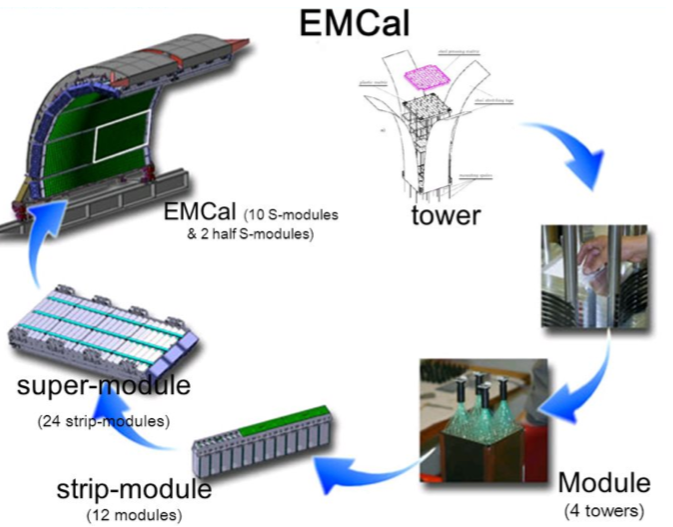
\includegraphics[width=12.0cm]{ALICEEMCAL}
\centering
\caption{ALICE EMCal along with super modules, tower strips, and towers\cite{1742-6596-110-3-032006}.}
\label{fig:EMCal}
\end{figure}


Figure \ref{fig:EMCal} shows the layout of the EMCal.  The smallest element of the EMCal is the `tower'\footnote{There are 12K towers in the EMCal}.  The tower serves as the readout and is made up of several layers of alternating scintillator and Pb-absorber.  Particles that interact via the electromagnetic force initiate a shower in the absorber material in the tower.  This electromagnetic shower induces light in the scintillator  to accumulate in the avalanche photodiodes in proportion to the particle's energy.  A `module' is an array of four towers that share readout electronics.  Twelve modules are placed in a single strip that provides support to the structure.  The largest component of the EMCal is the super-module, consisting of 1,100 towers,  which serves as the mounting structure to the ALICE detector.  The super-modules span a 20 degree angle in azimuth and ALICE currently has 10 full sized super-modlues and two 1/3 size super modules.  A second calorimeter was installed in 2015, the Dijet Calorimeter(DCAL), and allows for back-to-back jet measurements.


\subsubsection{EMCal Performance}
As particles enter the EMCal they initiate an electromagnetic shower.  The shower of electromagnetic particles spans several neighboring towers, these towers are grouped together into `clusters' and the Analog-To-Digital Conversion signal from the clusters corresponds to the energy deposited by the particle.  The EMCal was designed so that photons and electrons will fully shower inside of the tower region and thus fully deposit their energy.  Hadrons on the other hand will usually punch through the EMCal and only deposit a small fraction of their energy. 

 PID can be performed using the EMCal via track-cluster matching from the TPC.  TPC tracks are geometrically matched to the centroid of a cluster and if no track is matched, the cluster originated from a photon. If a track is matched, then the ratio of E/P, the energy of a matched cluster to the momentum of a TPC track, can be used to separate electrons from hadrons.

The energy resolution of the EMCal follows the form seen in Equation \ref{eq:emcalres}



\begin{equation}
\frac{\sigma}{E} = \sqrt{ A^{2} + \frac{B^{2}}{E} + \frac{C^{2}}{E^{2}}  }
\label{eq:emcalres}
\end{equation}

\noindent
where E is the cluster energy, A characterizes stochastic fluctuations such as photon collection efficiency, B is a function of the systematic effects such as detector non-uniformity, and C is a function of the noise in the Front-End Electronics (FEE). 

\begin{figure}[h]
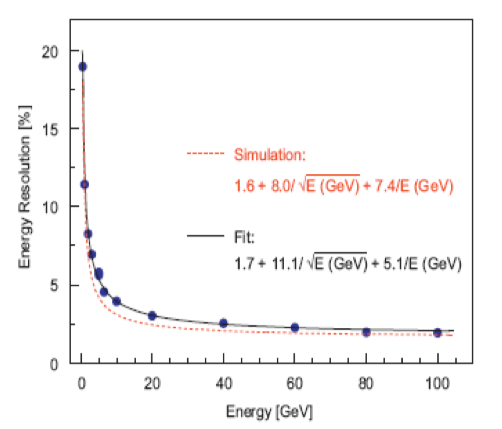
\includegraphics[width=11.0cm]{Alice-EMCal-Performance}
\centering
\caption{Energy resolution in the EMCal measured in a 2007 test beam at CERN (blue) compared to GEANT3 simulations of the EMCal (orange), fits for the parameters A, B, and C are also shown\cite{Abeysekara:2010ze}.}
\label{fig:EMCalres}
\end{figure}


As seen in Figure \ref{fig:EMCalres}, excellent agreement exits between the measured performance of the EMCal compared to simulations in a kinematic range between 10 GeV - 100 GeV and the resolution improves as the particle energy increases.  The stochastic term, A, is the largest source of uncertainty in the energy resolution in the EMCal.  Unlike the TPC, the resolution improves at high-$p_{t}$ making the EMCal ideal for measuring high energy particles and jets.


\subsubsection{EMCal Trigger}


Due to the high luminosity in the LHC, only a small fraction of events may be recorded to disk for later analysis.  ALICE employs a variety of triggers to record events that have the highest value for performing quality physics analysis.  The EMCal can trigger on events in order to increase the effective sample size for high-$p_{T}$ jets, photons, and electrons.  The two main triggers\cite{bourrion2010level}\cite{bourrion2013alice} for the EMCal are a jet trigger and a gamma trigger.  The gamma trigger is comprised of a 4x4 patch of EMCal towers, while the jet trigger is a 16x16 patch of towers.  Once the gamma trigger has surpassed a minimum energy threshold of 5 GeV\cite{Kral2012261} the event is tagged as a gamma event and the patch location is recorded.  EMCal jet triggered events have an energy threshold of 20 GeV and are similarly tagged and recorded.  The 5 GeV and 20 GeV thresholds used to fire the EMCal triggers are not fixed and the values quoted are specific to the 2012 8 TeV data set. 

\begin{figure}[h]
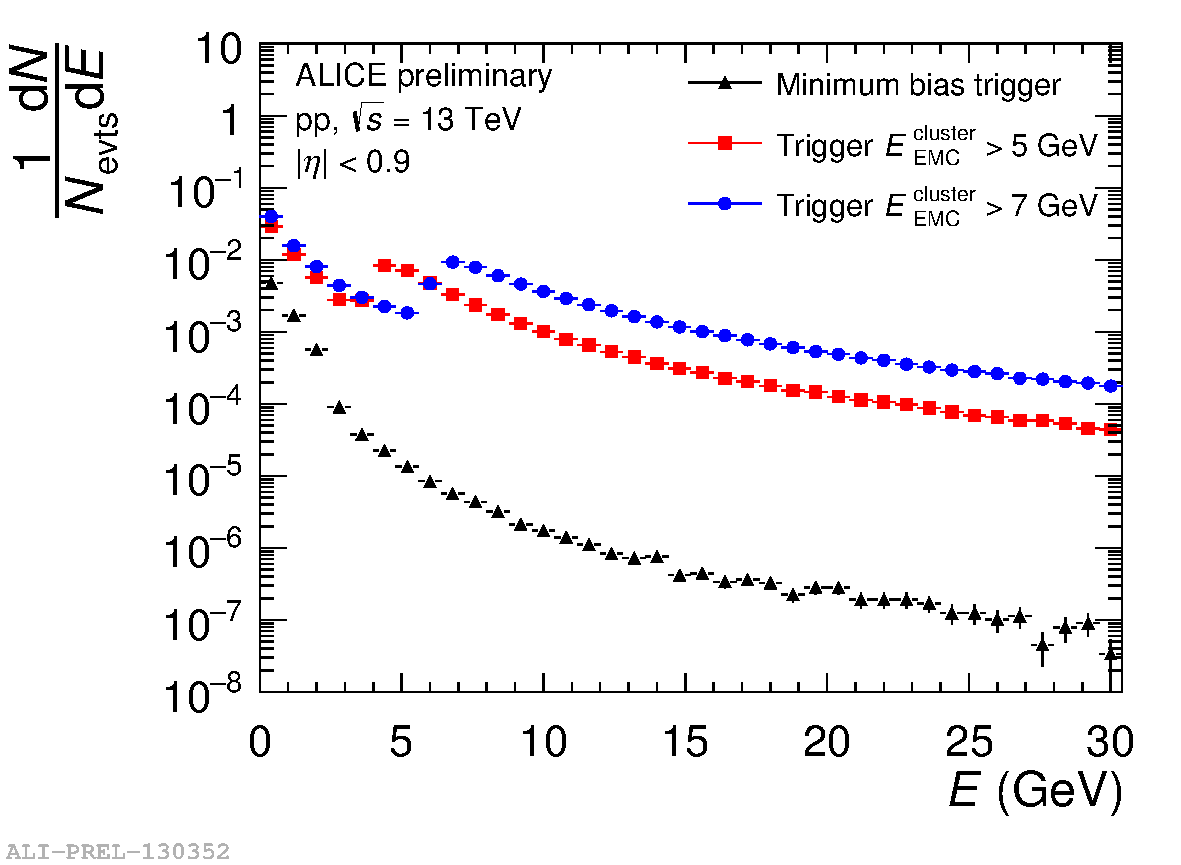
\includegraphics[width=12.0cm]{2017-Jul-05-Ecluster_emcal_alice_style}
\centering
\caption{Cluster Spectra from the ALICE EMCal.  MinBias is shown in black while the red and blue points show the spectra using the gamma trigger at two energy thresholds\cite{Jahnke:2018mrq}.}
\label{fig:EMCalSpectra}
\end{figure}

Figure \ref{fig:EMCalSpectra} shows the spectra from clusters measured in the EMCal using MinBias data in black and the gamma trigger from the EMCal set to two thresholds, 5 GeV and 7 GeV.  Recording the events that satisfy the EMCal triggers introduces a bias towards high-$p_{T}$ processes.  By using events that had an EMCal trigger, we can extend the kinematic range of an inclusive jet measurement, as seen in Figure \ref{fig:EMCalSpectra}.  In order to account for this bias it is necessary to calculate a trigger efficiency by comparing spectra from inclusive jets recorded using the MinBias trigger to the spectra generated from the EMCal triggers in the 8 TeV data set.  The calculation of the trigger efficiency will be discussed in depth in Chapter \ref{ch:analysis}.